\documentclass{article}

\usepackage{fancyhdr}
\usepackage{extramarks}
\usepackage{amsmath}
\usepackage{amsthm}
\usepackage{amsfonts}
\usepackage{tikz}
\usepackage[plain]{algorithm}
\usepackage{algpseudocode}
\usepackage{graphicx}

\usetikzlibrary{automata,positioning}

%
% Basic Document Settings
%

\topmargin=-0.45in
\evensidemargin=0in
\oddsidemargin=0in
\textwidth=6.5in
\textheight=9.0in
\headsep=0.25in

\linespread{1.1}

\pagestyle{fancy}
\lhead{Yousef Alaa Awad}
\chead{\hmwkClass\: \hmwkTitle}
\rhead{\firstxmark}
\lfoot{\lastxmark}
\cfoot{\thepage}

\renewcommand\headrulewidth{0.4pt}
\renewcommand\footrulewidth{0.4pt}

\setlength\parindent{0pt}

%
% Create Problem Sections
%

\setcounter{secnumdepth}{0}
\newcounter{partCounter}
\newcounter{homeworkProblemCounter}
\setcounter{homeworkProblemCounter}{1}

\newcommand{\hmwkTitle}{Homework\ \#1}
\newcommand{\hmwkDueDate}{February 3, 2026}
\newcommand{\hmwkClass}{Electronics 1}

%
% Title Page
%

\title{
    \vspace{2in}
    \textmd{\textbf{\hmwkClass:\ \hmwkTitle}}\\
    \normalsize\vspace{0.1in}
    \vspace{3in}
}

\author{Yousef Alaa Awad}

% Problems start here
\begin{document}

\maketitle
\pagebreak

\section{1.34}
\subsection{A) A germanium pn junction has a diode current of $I_D = 1.5 mA$ when biased at $V_D = 0.30 V$. What is the reverse bias saturation current?}
First we must find out the general formula for $I_S$.
$$ I_D = I_S*(e^{\frac{V_D}{V_T}}-1) \rightarrow I_S = \frac{I_D}{e^{\frac{V_D}{V_T}}-1} $$
After that, now we can substitute our numbers and simply solve!
$$ I_S = \frac{I_D}{e^{\frac{V_D}{V_T}}-1} \rightarrow I_S = \frac{1.5*10^{-3}}{e^{\frac{0.30}{0.026}}-1} \approx 1.462*10^{-8}A \rightarrow 14.62nA $$

\subsection{B) Using the results of part A, determine the diode current when the diode is biased at the following values.}
\subsubsection{VD = 0.35V}
$$ I_S = \frac{I_D}{e^{\frac{V_D}{V_T}}-1} \rightarrow I_S = \frac{1.462*10^{-8}}{e^{\frac{0.35}{0.026}}-1} \approx 10.3*10^{-3}A \rightarrow 10.3mA $$

\subsubsection{VD = 0.25V}
$$ I_S = \frac{I_D}{e^{\frac{V_D}{V_T}}-1} \rightarrow I_S = \frac{1.462*10^{-8}}{e^{\frac{0.25}{0.026}}-1} \approx 2.19*10^{-4}A \rightarrow 0.219mA $$


\pagebreak
\section{1.42}
\begin{figure}[!ht]
  \centering
  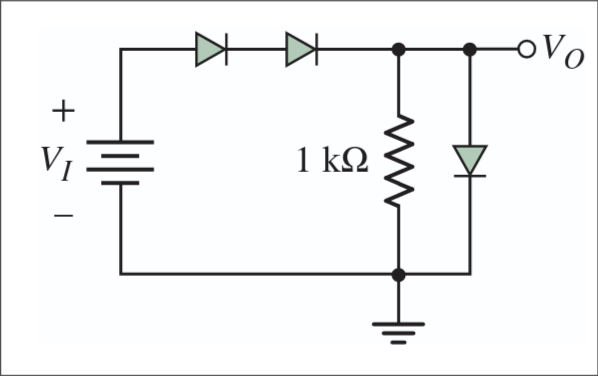
\includegraphics[width=0.5\textwidth]{p1_42.png}
  \caption{P1.42 from the textbook}
\end{figure}
\subsection{A) The reverse saturation current of each diode in the circuit shown in Figure P1.42 is $I_S = 6*10^{-14} A$. Determine the input voltage $V_I$ required to produce an output voltage of $V_O = 0.635 V$.}
$$ I_{D3} = (6*10^{-14})*e^{\frac{0.635}{0.026}} = 2.426mA $$
$$ I_{R} = \frac{0.635}{1} = 0.635mA $$
$$ I_{D1} = I_{D2} = 2.426 + 0.635 = 3.061mA $$
$$ V_{D1} = V_{D2} = 0.026*ln(\frac{0.003061}{6*10^{-14}}) = 0.641044V $$
$$ V_{in} = 2*V_D + V_O = 2*(0.664044)+0.635 = 1.917V $$

\subsection{B) Repeat part A if the 1 k$\Omega$ resistor is changed to $R = 500\Omega$.}
$$ I_{D3} = I_S*(e^{\frac{V_O}{V_t}} - 1) = 6*10^{-14}*(e^{\frac{0.635}{0.026}}-1) = 0.002426A $$
$$ I_R = \frac{V_O}{R_1} = \frac{0.635}{500} =0.001270A $$
$$ I_{in} = I_R + I_{D3} = 0.003696A = I_D $$
$$ V_D = V_T*ln(\frac{I_D}{I_S}) = 0.026*ln(\frac{0.003061}{6*10^{-14}}) = 0.645945V $$
$$ V_in = 2*V_D + V_O = 2*(0.645645) + 0.635 = 1.9269V $$

\pagebreak
\section{1.45}
The diode cut in voltage is $V_y = 0.7 V$ for the circuits shown in Figure P1.45. Plot $V_O$ and $I_D$ versus $I_i$ over the range $0 \le I_i \le 2 mA$ for the circuit shown in the following figures.

\subsection{A)}
\begin{figure}[!ht]
  \centering
  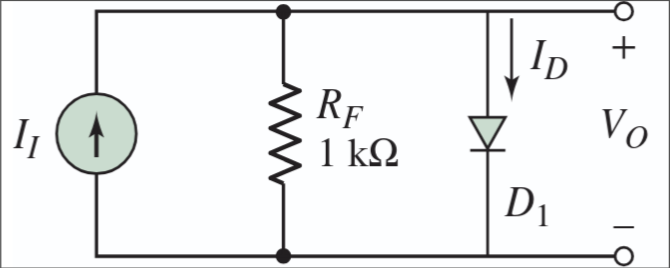
\includegraphics[width=0.5\textwidth]{p1_45a.png}
  \caption{P1.45a from the textbook}
\end{figure}
\[
V_O=
\begin{cases}
I_i, & 0 \le I_i \le 0.7mA \\
0.7,   & I_i \ge 0.7mA \\
\end{cases}
\]
\begin{figure}[!ht]
  \centering
  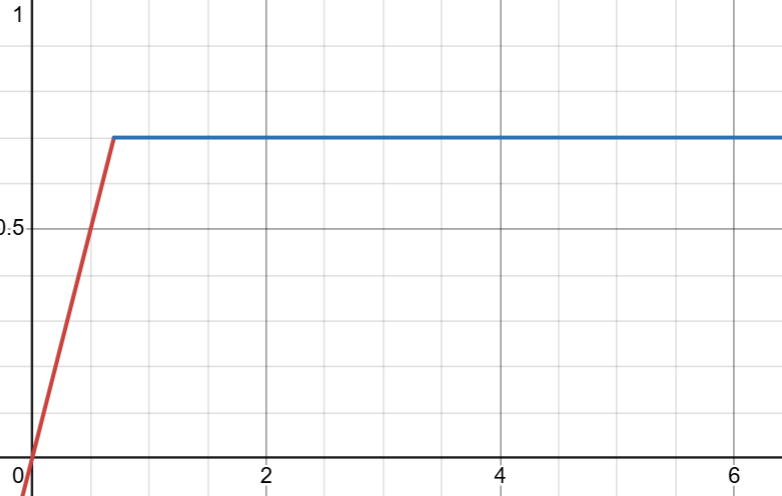
\includegraphics[width=0.5\textwidth]{p1_45answer_aa.png}
  \caption{Plot of $V_O$}
\end{figure}
\pagebreak
\[
I_D=
\begin{cases}
0,           & 0 \le I_i \le 0.7mA \\
I_i - 0.7,   & I_i \ge 0.7mA \\
\end{cases}
\]
\begin{figure}[!ht]
  \centering
  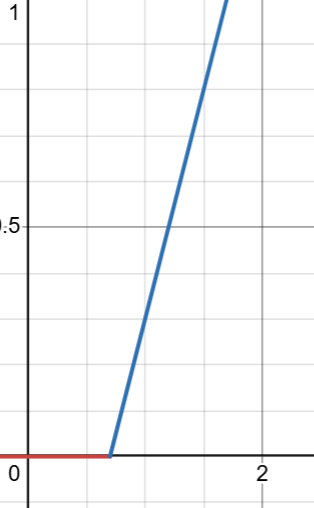
\includegraphics[width=0.5\textwidth]{p1_45answer_ab.png}
  \caption{Plot of $I_D$}
\end{figure}


\pagebreak
\subsection{B)}
\begin{figure}[!ht]
  \centering
  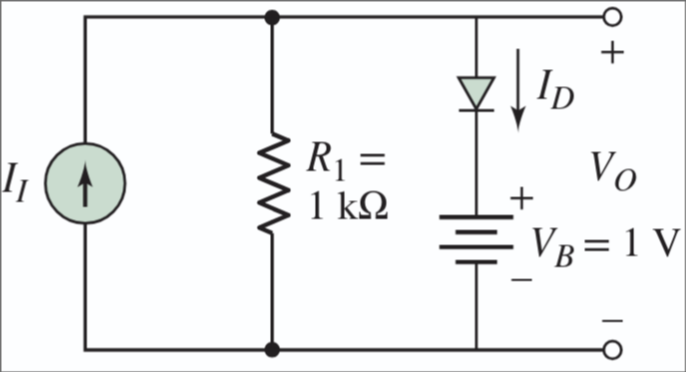
\includegraphics[width=0.5\textwidth]{p1_45b.png}
  \caption{P1.45b from the textbook}
\end{figure}
\[
V_O=
\begin{cases}
I_i, & 0 \le I_i \le 1.7mA \\
1.7,   & I_i \ge 1.7mA \\
\end{cases}
\]
\begin{figure}[!ht]
  \centering
  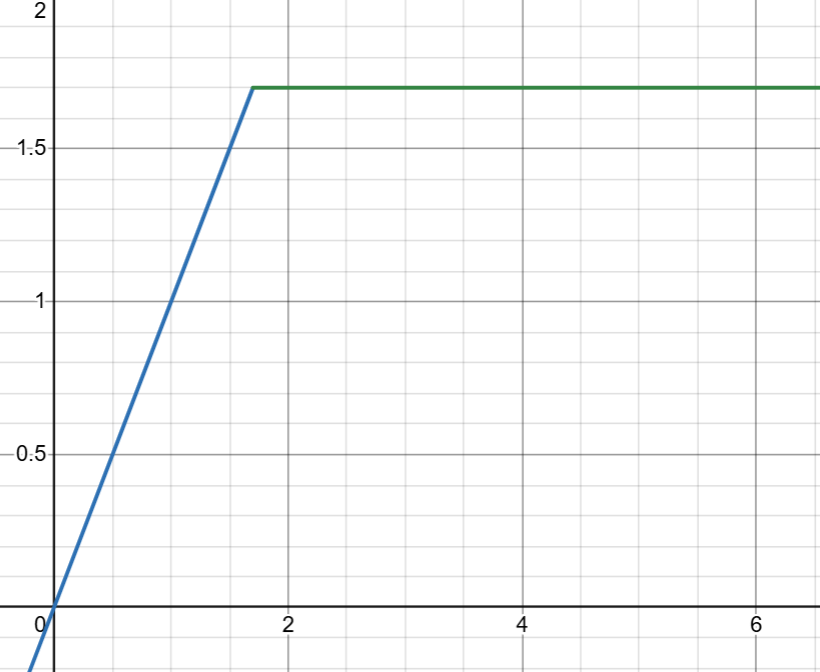
\includegraphics[width=0.5\textwidth]{p1_45answer_ba.png}
  \caption{Plot of $V_O$}
\end{figure}
\pagebreak
\[
I_D=
\begin{cases}
0,           & 0 \le I_i \le 1.7mA \\
I_i - 1.7,   & I_i \ge 1.7mA \\
\end{cases}
\]
\begin{figure}[!ht]
  \centering
  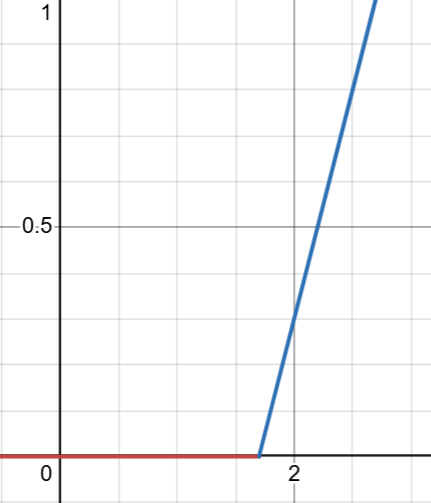
\includegraphics[width=0.5\textwidth]{p1_45answer_bb.png}
  \caption{Plot of $I_D$}
\end{figure}


\pagebreak
\subsection{C)}
\begin{figure}[!ht]
  \centering
  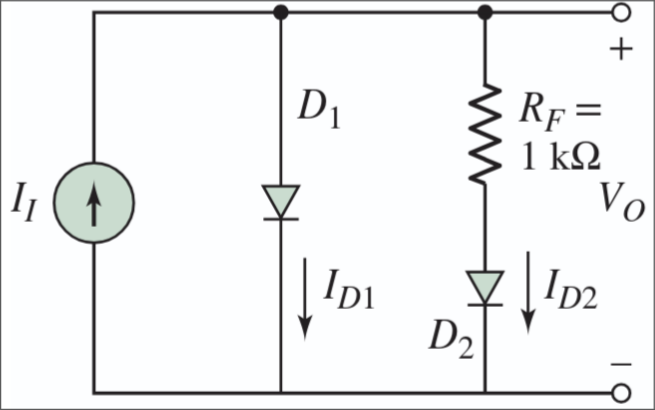
\includegraphics[width=0.5\textwidth]{p1_45c.png}
  \caption{P1.45c from the textbook}
\end{figure}
\[
V_O=
\begin{cases}
0,           & for\ all\ I_i \\
\end{cases}
\]
\begin{figure}[!ht]
  \centering
  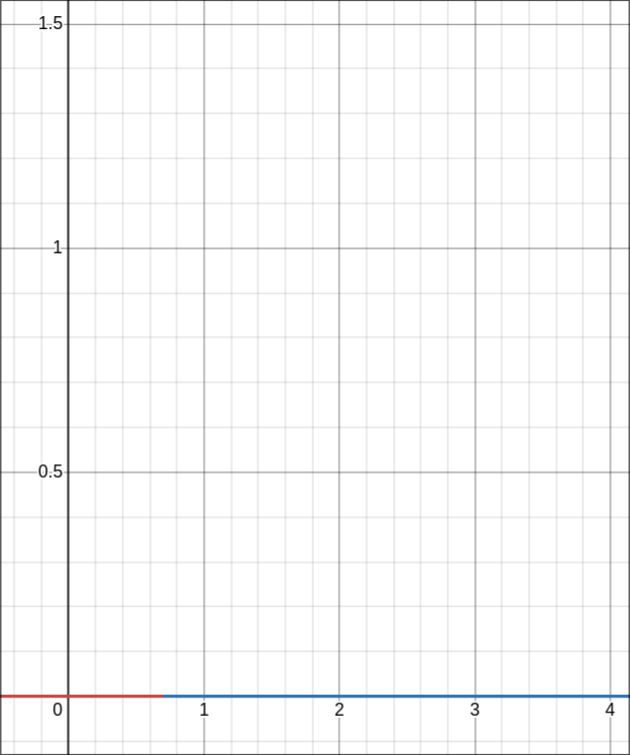
\includegraphics[width=0.5\textwidth]{p1_45answer_ca.png}
  \caption{Plot of $V_O$}
\end{figure}
\pagebreak
\[
I_D=
\begin{cases}
0,           & for\ all\ I_i \\
\end{cases}
\]
\begin{figure}[!ht]
  \centering
  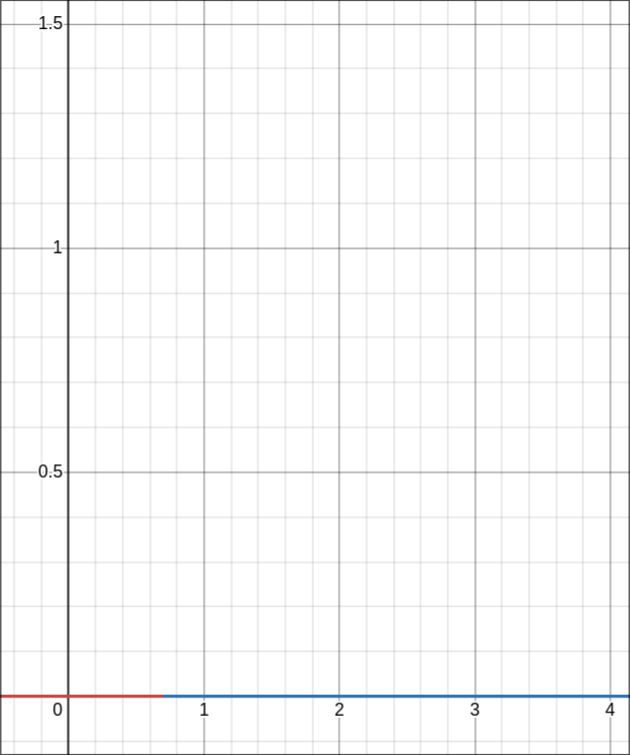
\includegraphics[width=0.5\textwidth]{p1_45answer_cb.png}
  \caption{Plot of $I_D$}
\end{figure}


\pagebreak
\section{1.50}
Assume each diode in the circuit shown in Figure P1.50 has a cut in voltage of $V_y = 0.65 V$.
\begin{figure}[!ht]
  \centering
  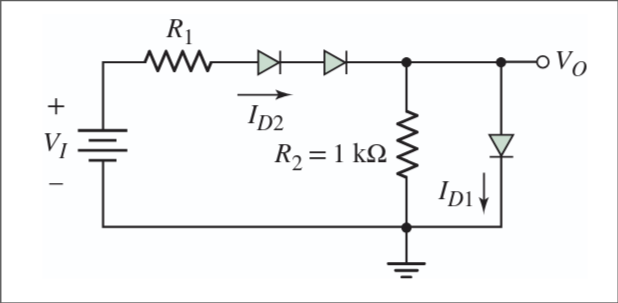
\includegraphics[width=0.5\textwidth]{p1_50.png}
  \caption{P1.50 from the textbook}
\end{figure}

\subsection{A) The input voltage is $V_I = 5 V$. Determine the value of $R_1$ required such that $I_{D1}$ is one half the value of $I_{D2}$. What are the values of $I_{D1}$ and $I_{D2}$?}
$$ I_{D1} = \frac{I_{D2}}{R_2} = \frac{0.65A}{1k\Omega} = 6.5*10^{-4} = 0.65mA $$
Given:
$$ I_{D1} = \frac{I_D2}{2} \rightarrow I_{D2} = 6.5*10^{-4}*2 = 1.3*10^{-4} = 1.3mA $$
Therefore...
$$ 5 - 0.0013*R_1 - 1.3 - 0.65 = 0 \rightarrow R_1 = 2346.15\Omega = 2.346k\Omega $$

\subsection{B) If $V_I = 8 V$ and $R1 = 2 \Omega$, determine $I_{D1}$ and $I_{D2}$.}
$$ 8V - V_{R1} - 2*0.65 - V_O = 0 \rightarrow $$
$$ 8V - I_{D2}*R_1 1.3 - V_O = 0 \rightarrow $$
$$ I_{D1} = I_{D2} - I_R \rightarrow $$
Therefore...
$$ I_{D2} = \frac{8-2*0.65-0.65}{2} = 3.025mA $$
$$ I_{D1} = I_{D2} -I_{R2} = 3.025 - \frac{0.65}{1000} = 2.375mA $$

\pagebreak
\section{1.51}
I will assume that n = 1 for the following math.

\subsection{A) Consider a pn junction diode biased at $I_{DQ} = 1 mA$. A sinusoidal voltage is superimposed on $V_{DQ}$ such that the peak to peak sinusoidal current is $0.05*I_{DQ}$. Find the value of the applied peak to peak sinusoidal voltage.}
Given:
$$ I_{DQ} = 1mA $$
$$ I_{pp} = 0.05*I_{DQ} = 0.05mA $$
Now, we do the following math (assuming the resistor is $R_d$):
$$ R_d = \frac{V_T}{I_{DQ}} = \frac{0.026}{0.001} = 26\Omega $$
And now we can use Ohm's law to find $V_{pp}$:
$$ V_{pp} = I_{pp}*R_d = 0.05*26 = 1.30mV $$

\subsection{B) Repeat part A assuming $I_{DQ} = 0.1 mA$.}
$$ I_{DQ} = 0.1mA $$
$$ I_{pp} = 0.05*I_{DQ} = 0.005mA $$
Now, we do the following math (assuming the resistor is $R_d$):
$$ R_d = \frac{V_T}{I_{DQ}} = \frac{0.026}{0.0001} = 260\Omega $$
And now we can use Ohm's law to find $V_{pp}$:
$$ V_{pp} = I_{pp}*R_d = 0.005*260 = 1.30mV $$


\end{document}

